%& -shell-escape

\documentclass{article}


\usepackage{amsmath}

\usepackage{mathtools,amssymb}
% math scr 
\usepackage{mathrsfs}  

\usepackage{pgfplots}
\pgfplotsset{width=7cm,compat=1.8}
\pgfmathdeclarefunction{gauss}{2}{%
  \pgfmathparse{1/(#2*sqrt(2*pi))*exp(-((x-#1)^2)/(2*#2^2))}%
}


\usepackage{graphicx}
\usepackage{python}

\begin{document}


\section*{Least squares}
Simple example
\begin{table}[!h]
\centering
\begin{tabular}{| c | c |}
\hline
\#  ($n$) & Ohms  ($y_n$) \\
\hline
1         & 1068        \\
2         & 988        \\
3         & 1002        \\
4         & 996        \\
\hline
\end{tabular}
\end{table}

the measurement model and the associated error

\begin{equation}
\begin{array}{ll}
{y_{1}=x+v_{1}} & {e_{1}^{2}=\left(y_{1}-x\right)^{2}} \\
 {y_{2}=x+v_{2}} & {e_{2}^{2}=\left(y_{2}-x\right)^{2}} \\
 {y_{3}=x+v_{3}} & {e_{3}^{2}=\left(y_{3}-x\right)^{2}} \\
 {y_{4}=x+v_{4}} & {e_{4}^{2}=\left(y_{4}-x\right)^{2}}
\end{array}
\end{equation}
minimizing the error

\begin{equation}
\hat{x}_{\mathrm{LS}}=\operatorname{argmin}_{x}\left(e_{1}^{2}+e_{2}^{2}+e_{3}^{2}+e_{4}^{2}\right)=\mathscr{L}_{\mathrm{LS}}(x)
\end{equation}

\begin{equation}
\begin{aligned} 
\mathbf{e} &= \left[\begin{array}{l}{e_{1}} \\ {e_{2}} \\ {e_{3}} \\ {e_{4}}\end{array}\right]  =\mathbf{y}-\mathbf{H} x \\
&=\left[\begin{array}{l}{y_{1}} \\ {y_{2}} \\ {y_{3}} \\ {y_{4}}\end{array}\right]-\left[\begin{array}{l}{1} \\ {1} \\ {1} \\ {1}\end{array}\right] x 
\end{aligned}
\end{equation}
Squared error, what we want to minimize

\begin{equation}
\begin{aligned} 
  \mathscr{L}_{\mathrm{LS}}(x)=e_{1}^{2}+e_{2}^{2}+e_{3}^{2}+e_{4}^{2} 
&=\mathbf{e}^{T} \mathbf{e} \\ &=(\mathbf{y}-\mathbf{H} x)^{T}(\mathbf{y}-\mathbf{H} x) 
\\ &=\mathbf{y}^{T} \mathbf{y}-x^{T} \mathbf{H}^{T} \mathbf{y}-\mathbf{y}^{T} \mathbf{H} x+x^{T} 
\mathbf{H}^{T} \mathbf{H} x 
\end{aligned}
\end{equation}
To get the smallest sol we do the derivative 

\begin{equation}
\begin{aligned}
{ \left.\frac{\partial \mathscr{L}}{\partial x}\right|_{x=\hat{x}}=-\mathbf{y}^{T} \mathbf{H}-\mathbf{y}^{T} \mathbf{H}+2 \hat{x}^{T} \mathbf{H}^{T} \mathbf{H}=0} \\
 {-2 \mathbf{y}^{T} \mathbf{H}+2 \hat{x}^{T} \mathbf{H}^{T} \mathbf{H}=0    }
\end{aligned}
\end{equation}
solving
\begin{equation}
  {\qquad \hat{x}_{\mathrm{LS}}=\left(\mathbf{H}^{T} \mathbf{H}\right)^{-1} \mathbf{H}^{T} \mathbf{y}}
\end{equation}
X hat minimizes our squared errors. Note: this is only possible if $H$ is not singular / has an inverse. This can be stated as the dimentions sadifying $n \geq m$, aka more mesurments than states.

\begin{equation}\mathbf{y}=\left[\begin{array}{c}{1068} \\ {988} \\ {1002} \\ {996}\end{array}\right] \quad \mathbf{H}=\left[\begin{array}{l}{1} \\ {1} \\ {1} \\ {1}\end{array}\right]
\end{equation}



\begin{equation}
\hat{x}_{\mathrm{LS}}=\left([11111]\left[\begin{array}{l}{1} \\ {1} \\ {1} \\ {1}\end{array}\right]\right)^{-1}[11111]\left[\begin{array}{c}{1068} \\ {988} \\ {1002} \\ {996}\end{array}\right] = 1013.5
\end{equation}



\section*{Weigted least squares}
We migt want to weight the mesurments because we 
might have better sensores that we trust more.


\begin{table}[!h]
\centering
\begin{tabular}{| l | c | c | }
\hline
\# & mulitmeter-A  ($\sigma=20$ Ohm) & mulitmeter-B  ($\sigma=2$Ohm) \\
\hline
1         & 1068 &       \\
2         & 988  &      \\
3         & &   1002      \\
4         & &     996 \\   
\hline
\end{tabular}
\end{table}



\begin{equation}
\begin{aligned}\left[\begin{array}{l}{y_{1}} \\ {\vdots} \\ {y_{m}}\end{array}\right] &=\mathbf{H}\left[\begin{array}{c}{x_{1}} \\ {\vdots} \\ {x_{n}}\end{array}\right]+\left[\begin{array}{c}{v_{1}} \\ {\vdots} \\ {v_{m}}\end{array}\right] \\ \mathbf{y} &=\mathbf{H x}+\mathbf{v} \end{aligned}
\end{equation}
Each time varying noiseterm $\mathbf{v_i}$ is an independent random variable across
 measurements and has an  an different  variance ( or standard deviation)
 accociated with it.



\begin{equation}
\mathrm{E}\left[v_{i}^{2}\right]=\sigma_{i}^{2}, \quad(i=1, \ldots, m) \quad \mathbf{R}=\mathbb{E}\left[\mathbf{v} \mathbf{v}^{T}\right]=\left[\begin{array}{ccc}{\sigma_{1}^{2}} & {} & {0} \\ {} & {\ddots} & {} \\ {0} & {} & {\sigma_{m}^{2}}\end{array}\right]
\end{equation}


Each squared error term is now weighted by the inverse of the variance associated with the corresponding measurement.

\begin{equation}
\begin{aligned} \mathscr{L}_{\mathrm{WLS}}(\mathbf{x}) &=\mathbf{e}^{T} \mathbf{R}^{-1} \mathbf{e} \\ &=\frac{e_{1}^{2}}{\sigma_{1}^{2}}+\frac{e_{2}^{2}}{\sigma_{2}^{2}}+\ldots+\frac{e_{m}^{2}}{\sigma_{m}^{2}} \end{aligned} \quad \text { where } \quad\left[\begin{array}{c}{e_{1}} \\ {\vdots} \\ {e_{m}}\end{array}\right]=\mathbf{e}=\left[\begin{array}{c}{y_{1}} \\ {\vdots} \\ {y_{m}}\end{array}\right]-\mathbf{H}\left[\begin{array}{c}{x_{1}} \\ {\vdots} \\ {x_{n}}\end{array}\right]
\end{equation}
We approach it's minimization the same way as before,

\begin{equation}
\begin{aligned} \mathscr{L}_{\mathrm{WLS}}(\mathbf{x}) &=\mathbf{e}^{T} \mathbf{R}^{-1} \mathbf{e} \\ &=(\mathbf{y}-\mathbf{H} \mathbf{x})^{T} \mathbf{R}^{-1}(\mathbf{y}-\mathbf{H} \mathbf{x}) \end{aligned}
\end{equation}
Solving in the same mannor

%\hat{\mathbf{x}}=\left.\operatorname{argmin}_{\mathbf{x}} \mathscr{L}(\mathbf{x}) \quad \longrightarrow \quad
\begin{equation}
  \begin{array}{c}
  \frac{\partial \mathscr{L}}{\partial \mathbf{x}}_{\mathbf{x}=\mathbf{\hat{x}}}
=\mathbf{0}=-\mathbf{y}^{T} \mathbf{R}^{-\mathbf{I}} \mathbf{H}+\hat{\mathbf{x}}^{T} 
\mathbf{H}^{T} \mathbf{R}^{-1} \mathbf{H} 
\end{array}
\end{equation}

\begin{equation}
 \mathbf{H}^{T} \mathbf{R}^{-1} \mathbf{H} \hat{\mathbf{x}}_{\text{WLS}}=\mathbf{H}^{T} \mathbf{R}^{-1} \mathbf{y}
\end{equation}
we get

\begin{equation}
\hat{\mathbf{x}}=\left(\mathbf{H}^{T} \mathbf{R}^{-1} \mathbf{H}\right)^{-1} \mathbf{H}^{T} \mathbf{R}^{-1} \mathbf{y}
\end{equation}






An example
\begin{equation}
\mathbf{H}=\left[\begin{array}{l}{1} \\ {1} \\ {1} \\ {1}\end{array}\right] \quad \mathbf{y}=\left[\begin{array}{c}{1068} \\ {988} \\ {1002} \\ {996}\end{array}\right] \quad \mathbf{R}=\left[\begin{array}{cccc}{\sigma_{1}^{2}} & {} & {} & {}  \\ {} &  {\sigma_{2}^{2}} & {}  & {} \\  {} & {} &  {\sigma_{3}^{2}} & {} \\ {} & {} & {} & {\sigma_{4}^{2}}\end{array}\right]=
\left[\begin{array}{cccc}{400} & {}  & {}  & {} \\ 
                         {} & {400}  & {}   & {}  \\ 
                         {} & {} & {4} & {}  \\ 
                         {} & {} & {} & {4}
\end{array}\right]
\end{equation}

\begin{equation}
\begin{aligned} \hat{x}_{\mathrm{WLS}} &=\left(\mathbf{H}^{T} \mathbf{R}^{-1} \mathbf{H}\right)^{-1} \mathbf{H}^{T} \mathbf{R}^{-1} \mathbf{y} \\ &=\left([1111]\left[\begin{array}{cccc}{400} & {}  & {}  & {} \\ 
                         {} & {400}  & {}   & {}  \\ 
                         {} & {} & {4} & {}  \\ 
                         {} & {} & {} & {4}
\end{array}\right]^{-1}
\left[\begin{array}{l}{1} \\ {1} \\ {1} \\ {1}\end{array}\right]
\right)^{-1}[11111]\left[\begin{array}{cccc}{400} & {}  & {}  & {} \\ 
                         {} & {400}  & {}   & {}  \\ 
                         {} & {} & {4} & {}  \\ 
                         {} & {} & {} & {4}
\end{array}\right]^{-1}\left[\begin{array}{c}{1068} \\ {988} \\ {1002} \\ {996}\end{array}\right] \\
 &= \frac{1}{1 / 400+1 / 400+1 / 4+1 / 4}\left(\frac{1068}{400}+\frac{988}{400}+\frac{1002}{4}+\frac{996}{4}\right) \\
 &= 999.3\end{aligned}
\end{equation}


Summery 

\begin{equation}
\begin{array}{cc}
{\mathscr{L}_{\mathrm{LS}}(\mathbf{x})=\mathbf{e}^{T} \mathbf{e}} & 
{\mathscr{L}_{\mathrm{WLS}}(\mathbf{x})=\mathbf{e}^{T} \mathbf{R}^{-1} \mathbf{e}} \\
 {\hat{\mathbf{x}}_{\mathrm{LS}}=\left(\mathbf{H}^{T} \mathbf{H}\right)^{-1} \mathbf{H}^{T} \mathbf{y}} 
& {\hat{\mathbf{x}}_{\mathrm{WLS}}=\left(\mathbf{H}^{T} \mathbf{R}^{-1} \mathbf{H}\right)^{-1} \mathbf{H}^{T} 
\mathbf{R}^{-1} \mathbf{y}} \\ {m \geq n} & {m \geq n} \\ {} & {\sigma_{i}^{2}>0}
\end{array}
\end{equation}








\begin{table}[h!]
\begin{tabular}{| l | l |}
\hline
Current (A) & Voltage (V) \\
\hline
0.2         & 1.23        \\
0.3         & 1.38        \\
0.4         & 2.06        \\
0.5         & 2.47        \\
0.6         & 3.17       \\
\hline
\end{tabular}
\end{table}
\newpage


\section*{Recursive Least Squares}
Teqniue that can be used when you dont want to compute the whole badge at a time.
\begin{equation}
\begin{aligned} \mathscr{L}_{\mathrm{RLS}} &=\mathbb{E}\left[\left(x_{k}-\hat{x}_{k}\right)^{2}\right] \\ &=\sigma_{k}^{2} \end{aligned}
\end{equation}
Generalizing this to the sates $n$
\begin{equation}
\begin{aligned} \mathscr{L}_{\mathrm{RIS}} &=\mathbb{E}\left[\left(x_{1 k}-\hat{x}_{1 k}\right)^{2}+\ldots+\left(x_{n k}-\hat{x}_{n k}\right)^{2}\right] \\ &=\operatorname{Trace}\left(\mathbf{P}_{k}\right) \end{aligned}
\end{equation}
$\mathbf{P}_{k}$ is the state covariance matrix. We can forumate a recursive
deeition of this $\mathbf{P}_{k}$ as a funciton of $\mathbf{K}_{k}$, by using matrix 
calculus and derivatives
\begin{equation}
\mathbf{P}_{k}=\left(\mathbf{1}-\mathbf{K}_{k} \mathbf{H}_{k}\right) \mathbf{P}_{k-1}\left(\mathbf{1}-\mathbf{K}_{k} \mathbf{H}_{k}\right)^{T}+\mathbf{K}_{k} \mathbf{R}_{k} \mathbf{K}_{k}^{T}
\end{equation}

\begin{equation}
\mathbf{K}_{k}=\mathbf{P}_{k-1} \mathbf{H}_{k}^{T}\left(\mathbf{H}_{k} \mathbf{P}_{k-1} \mathbf{H}_{k}^{T}+\mathbf{R}_{k}\right)^{-1}
\end{equation}

\begin{equation}
\begin{aligned} \mathbf{P}_{k} &=\mathbf{P}_{k-1}-\mathbf{K}_{k} \mathbf{H}_{k} \mathbf{P}_{k-1} \\ &=\left(\mathbf{1}-\mathbf{K}_{k} \mathbf{H}_{k}\right) \mathbf{P}_{k-1} \end{aligned}
\end{equation}

The larger our gain matrix $\mathbf{H}$, the smaller our new estimator covariance will be. Intuitively, you can think of this gain matrix as balancing the information we get from our prior estimate and the information we receive from our new measurement. 


\subsubsection*{Algorithm}
\begin{enumerate}
\item We initialize the algorithm with estimate of our unknown parameters and a corresponding covariance matrix. This initial guess could come from the first measurement we take and the covariance could come from technical specifications.
\begin{equation}
\begin{aligned} \hat{\mathbf{x}}_{0} &=\mathbb{E}[\mathbf{x}] \\ \mathbf{P}_{0} &=\mathbb{E}\left[\left(\mathbf{x}-\hat{\mathbf{x}}_{0}\right)\left(\mathbf{x}-\hat{\mathbf{x}}_{0}\right)^{T}\right] \end{aligned}
\end{equation}
\item Set up our measurement model and pick values for our measurement covariance.
\begin{equation}
\mathbf{y}_{k}=\mathbf{H}_{k} \mathbf{x}+\mathbf{v}_{k}
\end{equation}

\item Update the estimate and the covariance:
\begin{equation}
\begin{aligned} \mathbf{K}_{k} &=\mathbf{P}_{k-1} \mathbf{H}_{k}^{T}\left(\mathbf{H}_{k} \mathbf{P}_{k-1} \mathbf{H}_{k}^{T}+\mathbf{R}_{k}\right)^{-1} \\ \hat{\mathbf{x}}_{k} &=\hat{\mathbf{x}}_{k-1}+\mathbf{K}_{k}\left(\mathbf{y}_{k}-\mathbf{H}_{k} \hat{\mathbf{x}}_{k-1}\right) \\ \mathbf{P}_{k} &=\left(\mathbf{1}-\mathbf{K}_{k} \mathbf{H}_{k}\right) \mathbf{P}_{k-1} 
\end{aligned}
\end{equation}

\end{enumerate}



\newpage

\section*{Least Squares, Method of Maximum Likelihood}
Ganger alle gausian med hverandere
\begin{equation}
\begin{aligned} p(\mathbf{y} | x) & \propto \mathcal{N}\left(y_{1} ; x, \sigma^{2}\right) \mathcal{N}\left(y_{2} ; x, \sigma^{2}\right) \times \ldots \times \mathcal{N}\left(y_{m} ; x, \sigma^{2}\right) \\ &=\frac{1}{\sqrt{(2 \pi)^{m} \sigma^{2 m}}} \exp \left(\frac{-\sum_{i=1}^{m}\left(y_{i}-x\right)^{2}}{2 \sigma^{2}}\right)
\end{aligned}
\end{equation}
Prøver vi å makisimere

\begin{equation}
\begin{aligned} \hat{x}_{\mathrm{MLE}} &=\underset{x}{\operatorname{argmax}} p(\mathbf{y} | x) \\ &=\underset{x}{\operatorname{argmax}} \log p(\mathbf{y} | x) \end{aligned}\end{equation}

Take the log and get something we are farmilliar
\begin{equation}
\log p(\mathbf{y} | x)=-\frac{1}{2 R}\left(\left(y_{1}-x\right)^{2}+\ldots+\left(y_{m}-x\right)^{2}\right)+C
\end{equation}

\begin{equation}
\hat{x}_{\mathrm{MLE}}=\underset{x}{\operatorname{argmin}} \frac{1}{2 \sigma^{2}}\left(\left(y_{1}-x\right)^{2}+\ldots+\left(y_{m}-x\right)^{2}\right)
\end{equation}
\begin{equation}
\hat{x}_{\mathrm{MLE}}=\underset{x}{\operatorname{argmin}} \frac{1}{2}\left(\frac{\left(y_{1}-x\right)^{2}}{\sigma_{1}^{2}}+\ldots+\frac{\left(y_{m}-x\right)^{2}}{\sigma_{m}^{2}}\right) 
\end{equation}
\begin{equation}
 \hat{x}_{\mathrm{MHE}}=\hat{x}_{\mathrm{LS}}=\underset{x}{\operatorname{argmin}} 
 \mathscr{L}_{\mathrm{LS}}(x)=\underset{x}{\operatorname{argmax}} \mathscr{S}_{\mathrm{MHE}}(x)
\end{equation}
Good, but sensetive for outliers

\newpage

\section*{Kalman}

\begin{figure}[h]
  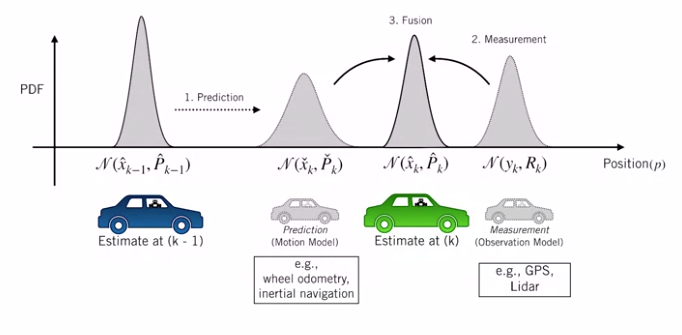
\includegraphics[width=\textwidth]{kalmanFig.png}
\end{figure}



\def\zright{1.645}%
\def\muzero{0}%
\def\muone{-1.95}%
\pgfplotsset{%
  myplot/.style={
    width=12cm,
    height=6cm,
%     xlabel=$z$, ylabel=$f(z)$,
    samples=50,
    legend style={draw=none, fill=none},
  }%
}%

\begin{figure}[!h]
\centering
\begin{tikzpicture}[%
  font=\scriptsize  ,
  >=stealth,
  every node/.style={rounded corners},
  Blue/.style={
    draw=none, text opacity=1, fill=blue!40!black, fill opacity=0.6
  },
  declare function={
    normalpdf(\x,\mu,\sigma)=
    (2*3.1415*\sigma^2)^(-0.5)*exp(-(\x-\mu)^2/(2*\sigma^2));
  }]

  \begin{axis}[myplot, hide axis]
    \addplot[Blue, draw, smooth, thick, domain=0:25]
    {normalpdf(x,3,0.5)};
    \node  at (30,-60) {$\mathcal{N}\left(\hat{x}_{k-1}, \hat{P}_{k-1}\right) $};
    \addplot[Blue, draw, smooth, thick, domain=0:25]
    {normalpdf(x,12,1)};
    \node  at (120,-60) {$ \mathcal{N}\left(\check{x}_{k}, \check{P}_{k}\right) $};
    \addplot[Blue, draw, smooth, thick, domain=0:25] 
    {normalpdf(x,18,0.55)} ;
    \node  at (180,-60) {$  \mathcal{N}\left(\hat{x}_{k}, \hat{P}_{k}\right) $};
    \addplot[Blue, draw, smooth, thick, domain=0:26]
    {normalpdf(x,22,0.7)} ;
    \node  at (223,-60) {$\mathcal{N}\left(y_{k}, R_{k}\right)$};

    \draw[->, smooth, thick] (0,0) -- (270,0) node[below] {$x$};
  \end{axis}
\end{tikzpicture}%
\end{figure}


\begin{figure}
\centering
\caption{$y(x)=\frac{\sin(x)}{x}$}
\end{figure}

\end{document}



  
